\documentclass[conference]{IEEEtran}
\usepackage{graphicx}
\usepackage{booktabs}
\usepackage{tabularx}
\usepackage{amsmath}
\usepackage{cite}
\usepackage{url}

\begin{document}

\title{GeoAD: Geometry-Aware Industrial Anomaly Detection from a Camera, More Accurate with a 3D Scanner}

\author{\IEEEauthorblockN{Adithya Chigullapally, Nikhil Sharma, Indraneel Ghosh}
\IEEEauthorblockA{Department of Computer Science and Engineering\\
Shiv Nadar University, India}}

\maketitle

\begin{abstract}
Visual inspection of manufactured parts is increasingly automated with anomaly detectors that learn what a normal part looks like. Methods that use only colour images miss many shape defects, and the strongest results on the MVTec 3D-AD benchmark come from methods that add an industrial 3D sensor. This report surveys four families of industrial anomaly detection: memory-bank methods on colour images, supervised segmentation-aware methods, colour-plus-3D methods, and vision-language foundation-model methods. We compare them on supervision, sensor requirements and reported accuracy, and identify three gaps. From these gaps we propose GeoAD, which combines Segment Anything, the segmentation-aware SegAD detector with PatchCore anomaly maps computed on WideResNet, DINO and CLIP features, and a vision-language model that describes each detected defect, and which adds a detector on measured depth when a 3D scanner is available. Preliminary experiments on MVTec 3D-AD reach 87.5 image-level AUROC from a camera alone (from 78.6 for SegAD on the whole image) and 92.1 when scanner depth is added.
\end{abstract}

\begin{IEEEkeywords}
industrial anomaly detection, defect inspection, foundation models, segmentation, 3D anomaly detection, explainability
\end{IEEEkeywords}

\section{Introduction}
\subsection{Background}
Industrial image anomaly detection (IAD) decides whether a manufactured part is defective and where the defect is. Defective parts are rare and varied, so most methods are trained on normal images only and flag anything that deviates from them~\cite{survey}. Memory-bank methods such as PatchCore~\cite{patchcore} store features of normal image patches from an ImageNet-pretrained network and score each test patch by its distance to the nearest stored patch; this reaches up to 99.6\% image-level AUROC on the MVTec AD benchmark.

\subsection{Motivation}
Colour images do not show every defect. The MVTec 3D-AD dataset~\cite{mvtec3d} pairs each colour image with a scan from a high-resolution industrial 3D sensor, and on it colour-only PatchCore reaches 78.5 image-level AUROC, while adding 3D point-cloud features raises this to 86.5 (BTF~\cite{btf}) and 94.5 (M3DM~\cite{m3dm}). A 3D sensor, however, adds cost, calibration and a second data pipeline, so many inspection stations have only a camera while others also have a scanner. Existing methods are built for one fixed setup: colour-only methods cannot use a scanner when it exists, and colour-plus-3D methods cannot run without one. A single detector that works from a camera alone, becomes more accurate when 3D data is available, and tells an operator \emph{what} is wrong rather than only returning a score, would fit both kinds of station.

\section{Research Problem}
Can one anomaly-detection pipeline detect and localise defects on manufactured parts from a fixed colour camera alone, become more accurate when an industrial 3D scanner is also available, and explain each detected defect in plain language?

\section{Objectives of the Literature Survey}
\begin{enumerate}
\item Categorise current IAD approaches by supervision and sensing modality.
\item Compare their accuracy on a common benchmark (MVTec 3D-AD) where results exist, and their data and hardware requirements.
\item Analyse critically why colour-only methods fall behind 3D methods, which recent foundation models could narrow that gap, and whether methods can use 3D data when present without depending on it.
\item Identify research gaps and define a research direction and research questions.
\end{enumerate}

\section{Literature Search Methodology}
We searched CVF Open Access (CVPR, ICCV), PMLR (ICML), OpenReview (ICLR), the AAAI proceedings and arXiv for work from 2021 to 2025, and verified every arXiv identifier against the arXiv API. Keywords were \emph{industrial anomaly detection}, \emph{MVTec 3D-AD}, \emph{supervised anomaly detection segmentation}, \emph{memory bank PatchCore}, \emph{multimodal RGB point cloud anomaly detection}, \emph{zero-shot anomaly detection CLIP}, \emph{multimodal large language model anomaly detection} and \emph{monocular depth estimation}. We included a paper if it reports results on an industrial benchmark (MVTec AD, MVTec 3D-AD, VisA) or provides a component used in our pipeline. We prioritised top-tier venues (CVPR, ICCV, ICML, ICLR, NeurIPS, AAAI), a peer-reviewed survey~\cite{survey}, and highly cited foundational papers, and kept 17 papers.

\section{Review of Existing Literature}
Following the taxonomy of Liu et al.~\cite{survey}, we group the literature into four approaches.

\subsection{Approach 1: Memory-bank detection on colour images}
PatchCore~\cite{patchcore} (CVPR 2022) extracts mid-level features of a WideResNet-50 pretrained on ImageNet, keeps a coreset-subsampled memory bank of normal patches, and uses nearest-neighbour distance as the anomaly score. It needs only normal images and localises defects through its patch-wise anomaly map. It is the colour baseline in most 3D work~\cite{btf,m3dm}.

\subsection{Approach 2: Supervised, segmentation-aware detection}
SegAD~\cite{segad} (CVPR 2024) targets complex parts made of several components. It splits the anomaly maps of one or more detectors into segments of the part, computes statistics per segment (99.5th percentile, skewness, kurtosis, mean), and feeds them to a boosted random forest (XGBoost) trained on normal images and a small number of defective images (10 in its VisA benchmark). It improves the state of the art on the Valeo Anomaly Dataset by 2.1 AUROC and on VisA by 0.4 (98.4). Its segment maps are static for aligned parts; for VisA they are object/background masks produced by Segment Anything (SAM)~\cite{sam}.

\subsection{Approach 3: Colour plus 3D sensing}
BTF~\cite{btf} shows that hand-crafted rotation-invariant point-cloud features (FPFH) outperform learned 3D features, and concatenating them with PatchCore colour features gives 86.5 image-level AUROC on MVTec 3D-AD. M3DM~\cite{m3dm} (CVPR 2023) uses DINO~\cite{dino} features for colour and Point-MAE features for point clouds, fuses them with a learned contrastive module and reaches 94.5; its colour-only branch alone reaches 85.0. Shape-Guided~\cite{shapeguided} (ICML 2023) keeps two memory banks, of local 3D shape and of colour features, and lets shape guide the anomaly scoring. Eyecandies~\cite{eyecandies} (ACCV 2022) is a second benchmark with colour, depth and normal maps.

\subsection{Approach 4: Vision-language foundation models}
CLIP~\cite{clip} learns aligned image and text features from 400 million image-text pairs. WinCLIP~\cite{winclip} (CVPR 2023) compares multi-scale image windows with an ensemble of text prompts describing normal and anomalous states, and reaches 91.8 image-level AUROC on MVTec AD with no training images, and 93.1 with one normal image. AnomalyCLIP~\cite{anomalyclip} (ICLR 2024) learns object-agnostic prompts and generalises across 17 industrial and medical datasets (91.5 zero-shot on MVTec AD). AnomalyGPT~\cite{anomalygpt} (AAAI 2024) feeds an image encoder and a localisation decoder into a large language model, which states in text whether an image is anomalous and where. MMAD~\cite{mmad} (ICLR 2025) benchmarks such multimodal models on 8,366 industrial images; the best (GPT-4o) reaches 74.9\% accuracy, far short of industrial requirements. General models such as Qwen3-VL~\cite{qwen3vl} describe images in free text but are not trained for defect detection.

\section{Comparative Analysis}
Table~\ref{tab:compare} summarises the approaches. Numbers come from the cited papers and follow their own protocols.

\begin{table*}[t]
\centering
\caption{Comparison of the reviewed approaches. I-AUROC: image-level AUROC on MVTec 3D-AD as reported in the cited paper (n/r: not reported; Approach 4 papers report MVTec AD only).}
\label{tab:compare}
\footnotesize
\setlength{\tabcolsep}{4pt}
\begin{tabularx}{\textwidth}{@{}p{2.2cm}p{2.6cm}p{2.4cm}p{2.4cm}p{1.3cm}X@{}}
\toprule
Approach & Representative & Training data & Input at test time & I-AUROC & Main limitation \\
\midrule
1 Memory bank & PatchCore~\cite{patchcore} & normal images & colour image & 78.5~\cite{btf} & ImageNet features, no shape information \\
2 Segmentation-aware & SegAD~\cite{segad} & normal + $\sim$10 defective & colour + segment map & n/r & needs segment maps; supervised \\
3 Colour + 3D & BTF~\cite{btf}, M3DM~\cite{m3dm} & normal images + scans & colour + point cloud & 86.5, 94.5 & industrial 3D sensor required \\
4 Vision-language & WinCLIP~\cite{winclip}, AnomalyCLIP~\cite{anomalyclip}, AnomalyGPT~\cite{anomalygpt} & none or few from the target product & colour + text & n/r & below trained methods; no 3D results \\
\bottomrule
\end{tabularx}
\end{table*}

\section{Critical Analysis}
\emph{Approach 1} is simple and needs no defective images, but ImageNet features suffer from ``feature drift'' on industrial images~\cite{survey}, and colour alone cannot reveal many geometric defects: depth-only PatchCore reaches only 63.7 and colour-only 78.5 on MVTec 3D-AD~\cite{btf}. \emph{Approach 2} exploits a few defective images and part structure, but its authors note that it requires segment maps, that static maps only suit aligned parts, and that its gain depends on object complexity~\cite{segad}; it has not been evaluated on a 3D benchmark. \emph{Approach 3} is the most accurate, but every result assumes an industrial 3D sensor and point-cloud processing, and the survey notes that current 3D methods cannot yet be deployed directly on real production data~\cite{survey}. Interestingly, M3DM's gain comes partly from better colour features: its DINO colour branch alone (85.0) already beats colour PatchCore (77.0 in its table). \emph{Approach 4} needs no training data, but zero-shot accuracy remains below trained detectors, and AnomalyCLIP observes that CLIP focuses on object class rather than abnormality~\cite{anomalyclip}. Approaches 1--3 return only scores and heatmaps. AnomalyGPT does explain defects in words, but there the language model also makes the decision, and MMAD shows that such models are not yet reliable inspectors~\cite{mmad}. Finally, reported numbers use different protocols (unsupervised, few-shot, supervised), so they are not directly comparable.

\section{Research Gaps}
\begin{enumerate}
\item[G1] Methods are designed for one fixed sensor setup, and no study measures, under the same pipeline and protocol, how much a camera-only detector loses against the same detector given a 3D sensor.
\item[G2] Segmentation-aware supervised detection (SegAD) uses ImageNet CNN detectors; self-supervised (DINO) and language-supervised (CLIP) features, strong in Approaches 3 and 4, have not been combined inside it, and SegAD has not been tested on MVTec 3D-AD.
\item[G3] Methods that explain defects in words let a language model decide~\cite{anomalygpt}, although such models are not reliable detectors~\cite{mmad}. We found no pipeline in which a trained detector decides and localises and a language model only describes the region it found.
\end{enumerate}

\section{Proposed Research Direction}
We propose GeoAD (Fig.~\ref{fig:pipeline}), a pipeline built from published components that runs in two modes. SAM~\cite{sam} separates object from background, as SegAD did for VisA~\cite{segad}. In \emph{camera mode}, PatchCore anomaly maps are computed on three feature extractors: WideResNet-50 (as in PatchCore), DINO ViT-B/8~\cite{dino} and CLIP ViT-B/16~\cite{clip} (layers 6 and 9). In \emph{3D mode}, when a scanner is available, a fourth PatchCore map is computed on the measured depth image. SegAD's per-segment statistics and boosted random forest combine whichever maps are available into a defect probability; each mode has its own head. When a part is flagged, the anomaly peak is boxed on the image and Qwen3-VL~\cite{qwen3vl} writes a one-sentence description of the boxed defect. The detector decides; the language model only describes.

\begin{figure}[t]
\centering
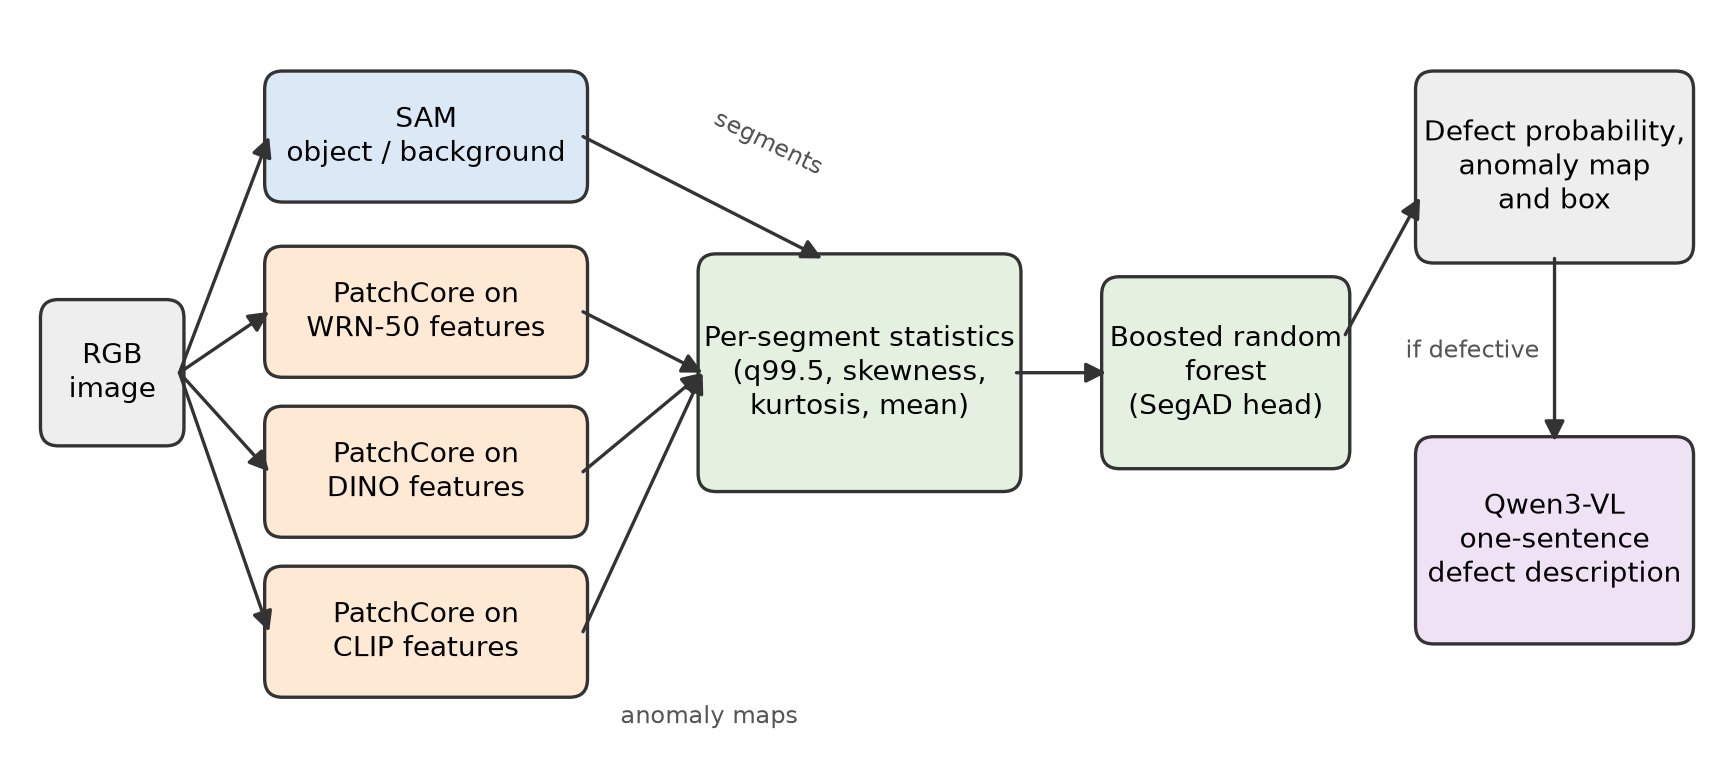
\includegraphics[width=\columnwidth]{fig_pipeline.png}
\caption{GeoAD in camera mode: SAM~\cite{sam} segments, PatchCore~\cite{patchcore} maps on WRN-50, DINO~\cite{dino} and CLIP~\cite{clip} features, the SegAD head~\cite{segad}, and Qwen3-VL~\cite{qwen3vl} for the description. 3D mode adds a PatchCore map on the scanner's depth image.}
\label{fig:pipeline}
\end{figure}

\subsection{Preliminary results}
We use the RGB images of MVTec 3D-AD~\cite{mvtec3d} (10 classes; 2656 training, 294 validation and 1197 test images) at 256$\times$256 pixels and SegAD's supervised protocol: for each of its 10 official seeds, the head is trained on validation images plus 10 randomly chosen defective test images and evaluated on the remaining test images. Table~\ref{tab:results} reports image-level AUROC (mean $\pm$ standard deviation over seeds). Because this protocol uses 10 defective images, the numbers are not comparable to the unsupervised results in Table~\ref{tab:compare}; the reference is our own run with real sensor depth under the same protocol. The seeds share the same test images, so we also compare adjacent rows seed by seed: every added component improves AUROC in all 10 seeds (SAM $+$3.8, DINO $+$2.8, CLIP $+$2.3, depth $+$4.6; paired standard deviation 0.8--1.2).

We first tried to replace the scanner with monocular depth from Depth Anything V2~\cite{dav2}, under the same protocol with the whole image as one segment. On geometric defects it moved AUROC only from 78.1 to 78.2, while real sensor depth reached 90.0, so estimated depth recovered about 1\% of the sensor's gain. This is why GeoAD uses stronger colour features instead of estimated depth.

\begin{table}[t]
\centering
\caption{Preliminary results on MVTec 3D-AD (image-level AUROC, 10 classes $\times$ 10 seeds, SegAD protocol).}
\label{tab:results}
\small
\begin{tabular}{lcc}
\toprule
Setup & 3D sensor & I-AUROC \\
\midrule
SegAD, whole image as one segment & no & 78.6 $\pm$ 1.2 \\
\quad + SAM object/background & no & 82.4 $\pm$ 0.9 \\
\quad + DINO detector & no & 85.2 $\pm$ 1.1 \\
\quad + CLIP detector (GeoAD, camera) & no & \textbf{87.5 $\pm$ 0.9} \\
\quad + real depth detector (GeoAD, 3D) & yes & \textbf{92.1 $\pm$ 1.3} \\
\midrule
SegAD (one segment) + real depth & yes & 90.3 $\pm$ 0.9 \\
\bottomrule
\end{tabular}
\end{table}

In camera mode GeoAD reaches 87.5 and improves geometric, surface and mixed defect groups alike (86.8, 87.5 and 87.2). Adding the scanner's depth raises it to 92.1. This is only 1.8 above SegAD with depth and one segment (90.3; higher in 9 of 10 seeds, paired standard deviation 1.2), so with a scanner most of the accuracy comes from the depth itself. Our 3D mode is also not state of the art: M3DM reaches 94.5 without any defective images~\cite{m3dm}. Depth helps most on objects with shape defects, such as potato (67.8 to 86.6), cookie (79.8 to 92.8) and cable gland (87.2 to 94.8). Camera mode recovers about two thirds of the gain of 3D mode over the one-segment baseline ((87.5$-$78.6)/(92.1$-$78.6)). Grouping SAM masks into colour-based part types did not help (78.7), cropping each image to the SAM object reduced AUROC (79.4 with WRN-50), and 384-pixel input reduced it as well (83.9 with WRN-50 and DINO). Fig.~\ref{fig:demo} shows a detected defect. The description here is correct in location but names the wrong type (``missing piece'' for a bent dowel). Measured on 316 held-out defective images, the box centre falls on the defect in only 37.7\% of cases and a keyword match finds the right type in 41.5\% (a lenient test), so the explanations are unreliable, and at threshold 0.5 some classes give many false alarms (tire 66\%, cookie 48\%). Each detector is also tied to its capture setup: camera mode was evaluated only on the scanner's own colour images, and on 74 phone photos of carrots from another source (different camera, lighting and variety) the carrot detector scored 45.2, chance level. GeoAD therefore suits a fixed inspection station and must be refitted for a new setup from its good images and about ten defective ones.

\begin{figure}[t]
\centering
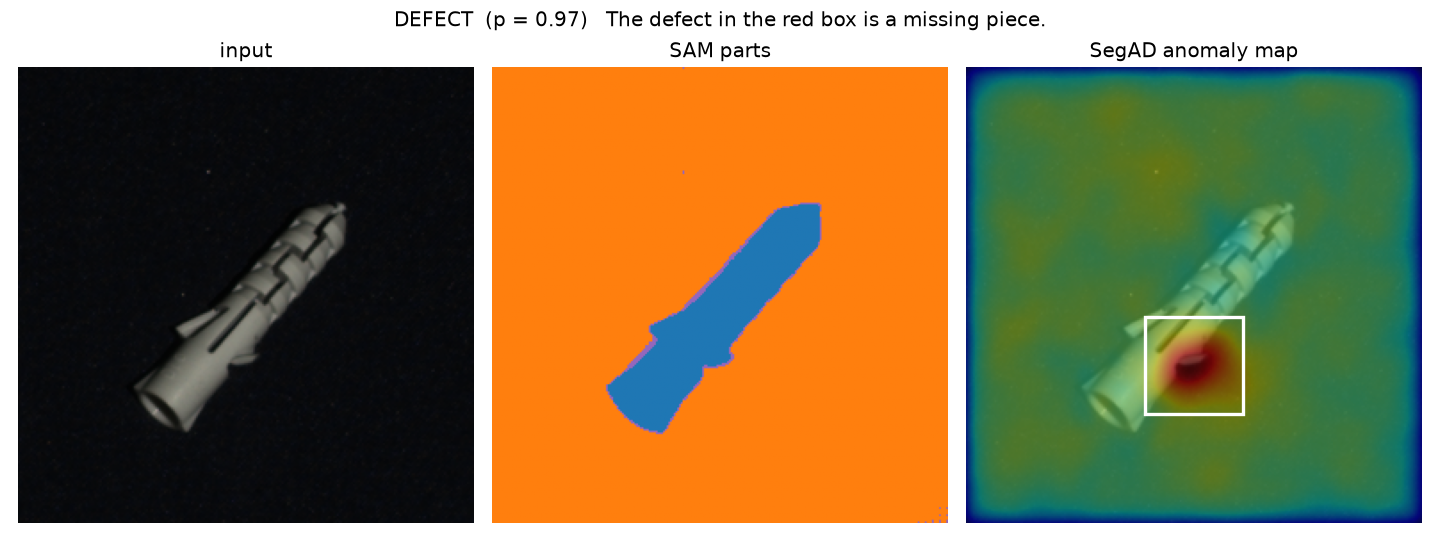
\includegraphics[width=\columnwidth]{fig_demo.png}
\caption{Output on an unseen defective dowel (ground truth: bent). Left to right: input, SAM segments, anomaly map with the box given to Qwen3-VL. Title: predicted probability and the generated description.}
\label{fig:demo}
\end{figure}

\section{Preliminary Research Questions}
\begin{enumerate}
\item[RQ1] How accurate is one segmentation-aware pipeline from a camera alone, how much more accurate does it become when a 3D scanner is added, and how much of that gap can foundation-model features close?
\item[RQ2] Are DINO and CLIP features complementary to ImageNet CNN features inside SegAD, and does this hold on a second dataset?
\item[RQ3] Can the explanation be made reliable? A 2B vision-language model named the right type in 41.5\% of cases, so what box, prompt or model would raise this?
\end{enumerate}

\section{Conclusion}
The literature shows a clear trade-off: colour-only detectors are cheap but miss shape defects, colour-plus-3D detectors are accurate but need an industrial sensor, and vision-language models are flexible but not yet reliable detectors. Our preliminary results suggest that one segmentation-aware pipeline can serve both kinds of inspection station: with foundation-model features it reaches 87.5 from a camera alone, and 92.1 when a 3D scanner is added, while depth estimated from a single photo does not replace the scanner. Next steps are to test both modes on a second dataset (VisA has colour only; Eyecandies~\cite{eyecandies} has colour and depth), to test refitting on a new capture setup, and to make the generated descriptions reliable, since they currently name the right defect type in only 41.5\% of cases.

\begin{thebibliography}{00}
\bibitem{survey} J. Liu, G. Xie, J. Wang, S. Li, C. Wang, F. Zheng and Y. Jin, ``Deep industrial image anomaly detection: A survey,'' \emph{Machine Intelligence Research}, vol. 21, no. 1, pp. 104--135, 2024.
\bibitem{patchcore} K. Roth, L. Pemula, J. Zepeda, B. Sch\"olkopf, T. Brox and P. Gehler, ``Towards total recall in industrial anomaly detection,'' in \emph{Proc. CVPR}, 2022.
\bibitem{mvtec3d} P. Bergmann, X. Jin, D. Sattlegger and C. Steger, ``The MVTec 3D-AD dataset for unsupervised 3D anomaly detection and localization,'' in \emph{Proc. VISAPP}, 2022.
\bibitem{btf} E. Horwitz and Y. Hoshen, ``Back to the feature: Classical 3D features are (almost) all you need for 3D anomaly detection,'' in \emph{Proc. CVPR Workshops}, 2023.
\bibitem{m3dm} Y. Wang, J. Peng, J. Zhang, R. Yi, Y. Wang and C. Wang, ``Multimodal industrial anomaly detection via hybrid fusion,'' in \emph{Proc. CVPR}, 2023.
\bibitem{segad} A. Baitieva, D. Hurych, V. Besnier and O. Bernard, ``Supervised anomaly detection for complex industrial images,'' in \emph{Proc. CVPR}, 2024.
\bibitem{sam} A. Kirillov \emph{et al.}, ``Segment anything,'' in \emph{Proc. ICCV}, 2023.
\bibitem{dino} M. Caron, H. Touvron, I. Misra, H. J\'egou, J. Mairal, P. Bojanowski and A. Joulin, ``Emerging properties in self-supervised vision transformers,'' in \emph{Proc. ICCV}, 2021.
\bibitem{clip} A. Radford \emph{et al.}, ``Learning transferable visual models from natural language supervision,'' in \emph{Proc. ICML}, 2021.
\bibitem{winclip} J. Jeong, Y. Zou, T. Kim, D. Zhang, A. Ravichandran and O. Dabeer, ``WinCLIP: Zero-/few-shot anomaly classification and segmentation,'' in \emph{Proc. CVPR}, 2023.
\bibitem{anomalyclip} Q. Zhou, G. Pang, Y. Tian, S. He and J. Chen, ``AnomalyCLIP: Object-agnostic prompt learning for zero-shot anomaly detection,'' in \emph{Proc. ICLR}, 2024.
\bibitem{qwen3vl} Qwen Team, ``Qwen3-VL technical report,'' arXiv:2511.21631, 2025.
\bibitem{shapeguided} Y.-M. Chu, C. Liu, T.-I. Hsieh, H.-T. Chen and T.-L. Liu, ``Shape-guided dual-memory learning for 3D anomaly detection,'' in \emph{Proc. ICML}, 2023.
\bibitem{eyecandies} L. Bonfiglioli, M. Toschi, D. Silvestri, N. Fioraio and D. De Gregorio, ``The Eyecandies dataset for unsupervised multimodal anomaly detection and localization,'' in \emph{Proc. ACCV}, 2022.
\bibitem{anomalygpt} Z. Gu, B. Zhu, G. Zhu, Y. Chen, M. Tang and J. Wang, ``AnomalyGPT: Detecting industrial anomalies using large vision-language models,'' in \emph{Proc. AAAI}, 2024.
\bibitem{mmad} X. Jiang \emph{et al.}, ``MMAD: A comprehensive benchmark for multimodal large language models in industrial anomaly detection,'' in \emph{Proc. ICLR}, 2025.
\bibitem{dav2} L. Yang, B. Kang, Z. Huang, Z. Zhao, X. Xu, J. Feng and H. Zhao, ``Depth Anything V2,'' in \emph{Proc. NeurIPS}, 2024.
\end{thebibliography}

\end{document}
